\documentclass[a4paper,12pt,fleqn,dvipsnames,oneside,openright]{memoir} 
%\usepackage[utf8]{inputenc}
%\usepackage{graphicx}
%\usepackage{pdfpages}
%\usepackage{setspace}
%\usepackage{geometry}
\usepackage{Preamble}

\addbibresource{references.bib} %Tilføjer kildeliste

\title{Artion}
\author{Mads, Lukas and Morten}
\date{December 2017}

\usepackage{graphicx}

\begin{document}
\maketitle

\section*{\centerline{Innovation and new technology}}

\newpage
\tableofcontents*
\thispagestyle{empty}
%\addtocontents{toc}{~\hfill\textbf{Side}\par}

\mainmatter 

\chapter{Introduction}
\section{Application}

\textbf{Penny Bid Auction with art} \\
Our application is the future of online painting auctions. Penny bid auctions are seen before and still exist in foreign countries, but we have made a twist on the concept. The concept of our application is to provide a platform for amateur artists or individuals to sell their paintings at low prices but with high earnings because of the penny bid concept.\\  

\textbf{Auctions and Prices}\\
The start price of an action is always 0 kr. Our idea of creating this platform is that prices are different from other similar platforms. If a potential buyer wants the product, the buyer has to submit a bid. One bid costs 5 kr. For each bid a potential buyer submit for a given painting, the price of the painting increases with 0,10 Kr. A bidder can submit as many bids as he wants, but he pays 5 kr. each time he submits a bid. Let's take an example: if an auction ends with a selling price at 100 kr., the earnings for the seller will be 5.100 kr.
\begin{equation}
Earnings = ((\frac{100}{0,10}) * 5)+100=5.100\ kr.
\end{equation}
The sellers profit primarily consists of the bidders bids at the given auction.\\

\textbf{Prices}
\begin{itemize}
    \item Opening price for an action: 0 kr.
    \item Raise in selling price per. submitted bid: 0,10 kr. (10 øre)
    \item Price per. bid: 5 kr.
\end{itemize}

Equation for the seller's earnings: 
\begin{equation}\label{sellersEarnings}
    Earnings = ((\frac{Selling\ price}{0,10}) * Bid\ price)+Selling\ price
\end{equation}

An auction automatically ends seven days after it is created. If a bid is submitted with less than two minutes left, the expiration time of the auction is extended to two minutes - this continues until no more bids are submitted. The last bidder buys the concerned painting. \\

The winner of an auction can in principle buy a painting for 5 kr. (bid price + selling price). On the other side, there might be many other bidders who pays to bid but don't actually buy the concerned painting.\\

\textbf{Advantages and the background of the project}\\
The concept behind the penny-bid-auction have, by ethical code, been a 'grey area'. We want to change that vision.\\

On previous penny-bid-auctions websites in Denmark, the companies themselves have been the seller of all products - therefore, private individuals couldn't sell their own paintings.\\

This has resulted in several examples where companies have implemented bid-robots, that aim to submit bids on auctions to raise the selling price and to encourage other users to submit more bids. In this way the company earns even more on an auction because they don't pay for the bids submitted by the robots, but they cheat other users to submit more bids.\\

We eliminate this problem by not being the seller of the products, in this case, paintings. In our application individuals are the sellers, therefore, it wouldn't be profitable for us to implement bid-robots.  \\

\textbf{Users}\\
We expect to have the following two types of users as our primary target group.\\

\begin{enumerate}
\item People who wants to gamble and get the opportunity to sell a painting and possibly get a higher earnings than they would get at a regular auction or sales advertisement.
Our concept allows the sellers to earn a lot more on a painting, than he could in comparison to other types of sales. This is spite of a very low selling price and a potentially cheap painting for the buyer. 

\textbf{Example}: A painting sold for 200 kr., gives the seller a profit of 10.200 Kr.\\
\item People who wants to gamble and get the opportunity to buy a painting at a lower price than they could on a regular auction or sales advertisement. 
Our concept allows the buyers to buy a given painting at a much cheaper price than he could find elsewhere. 

\textbf{Example}: Even if the seller has earned far above the expected selling price, the buyer will be able to buy the product for 5 Kr. (Bid price) + the likely low selling price.\\
\end{enumerate}

\textbf{Possible challenges}\\

\textbf{Idea for design and construction}\\
First side: Vertical list with all the auctions. From the top are the auctions who are about to expire. From there the user can choose categories or scroll down through the auctions.\\

\textbf{Terms of payment}\\
When an auction has ended, the amount of money paid by the bidders will be locked by the company. The seller will receive the money when both the seller and the buyer has confirmed the deal.\\  

\textbf{Terms of bids}\\

\chapter{Market environment - Lukas}
\section{Market Analysis}
The competition for auctions in the Danish market is widely different. There are from the major national auctions, to the small locals. Our idea focuses on paintings and being able to sell it online.
When we look at the major competitors in the market, we see companies like Lauritz.com and Brunn Rasmussen. Here the auctions take place only after an assessment of the individual products has taken place. The much more accessible company is DBA. Here it costs you nothing to create an ad and you hit a large segment of any buyers. However, you set a fixed price, but others have the opportunity to bid more or less than that.
We have conducted a market analysis based on earnings before tax, in order to categorise and rank our direct competitors in the market.
As we can see in annex X, where we have set up a table, with our competitors and ourselves, it can be highlighted that we certainly have a role to play in the Danish market.
With a calculation of the profit for the year at 304K DKK. we can determine that we earn more than 3 of our 4 competitors. There may be some investment reasons why the 2 competitors create a deficit in the current financial year.

\chapter{Innovation strategies}
\section{Innovation strategies}
\section{How do we enact these strategies?}
\section{Contributors}
\section{Input from contributors}

\chapter{Value proposition - Mads}
\section{Capability}
\subsubsection{Frame recognising camera}
\label{FrameCamera}
The frame recognising camera is one of the essential features that makes our application unique. When a user creates an auction, he must use the built-in camera function that recognises the frame of the painting and only captures what is within the frame. In this way we ensure a consistent presentation of all auctions. This process is illustrated in figure \ref{CreateAuction}.

\subsubsection{Simplicity}
One of the reasons for us to develop this app, is that the existing platforms at the current market are not simple and easy to use. Lauritz.com provides a quite easy and simple application. They manage all of the auctions, including valuation, picturing, storing in showrooms and distribution of products after hammering. We think Lauritz.com provides a simple and easy to use application, but the associated processes are very difficult for both the seller and the buyer, in terms of handling and pickup. 

\subsubsection{Safe transactions}
With inspiration from services like AirBnB and Uber, we introduce the transaction-confirmation feature. All transactions and payments are managed by the application. When an auction has ended, the payment is locked in the system. The seller will be notified when the buyer has payed for the product, but the seller will not receive any money before the painting is received by the buyer. We have implemented an interface that enables the buyer and seller to confirm that the exchange of the product has taken place, whereafter the seller receives the money.  
\section{Impact}
We think too many potential profitable paintings at DBA among other platforms are disappearing in the abundance of products. Currently at DBA in the category "Paintings" we find almost 13.500 advertisements\footnote{https://www.dba.dk/til-boligen/kunst-og-antikviteter/malerier/}. Most of these advertisements does not get any attention and ends up being lost in the crowd. Our application aims to bring them into the light, which it does in three ways; frame recognising camera, simplicity and seven days before expiration.\\ 
\forceindent The majority of the advertisements for paintings at DBA and QXL have really bad pictures, which results in less attention. Examples of the pictures and the presentation of advertisements at DBA and QXL, are illustrated in appendix \ref{CompetitorsPlatforms}. The frame recognising camera feature ensures the picture of a given painting is perfectly scaled and hereby presented in the best possible way. Another issue at DBA is that it does not by default sort the products by the expiration date, meaning the old and "bad" advertisements gets a bad location. \\

Artion benefits the market by providing a platform that makes it easy and quick to create advertisements with consistent and perfectly scaled pictures. Hereby ensuring equal spotlight for all advertisements by always sorting by expiration date and time. 
\section{Proof}
The primary evidence substantiating the value proposition of Artion, is the success of the existing platforms, from which we combine various fragments. The three major concepts we combine are as follows: 
\begin{enumerate}
    \item DBA: Quick and easy to create advertisements (short time to market)
    \item Lauritz.com: Consistent presentation of auctions and 7 days before expiration
    \item Instagram: User profiles with infinite scrolling 
\end{enumerate}
These are three well-established concepts, that has proven to be popular over many years. We consider the success of these concepts as the evidence substantiating the value proposition of Artion. We combine these concepts in order to meet the latent needs of consumers, who make up for a gap in the market, which is elaborated in chapter \ref{Market}.

\section{Cost}
The greatest costs we expect to face in relation to launching the application, are costs related to hosting, data storage, transactions and marketing. Firstly, we need to establish a partnership with a hosting company to take care of all technical aspects regarding hosting, maintenance, support and storing of data. The costs related to hosting is dependent on the amount of users, auctions, transactions and so fourth. Furthermore, we need an integration with a payment module, and a subscription for a payment solution. Finally, we need to invest in marketing the application and raise attention in order to attract users. The primary channel we plan to use for marketing is social media, hereby sponsored campaigns. 

\chapter{Value adding activities}

\chapter{User tasks}

\chapter{Design sketches}

\chapter{Key innovative featuresskipper.mbn94@gmail.com}


\chapter{Data handling}

\chapter{Business model}

\chapter{Commercial challenges}

\chapter{Screenshots}

\begingroup
	\raggedright
	\printbibliography
\endgroup 


\appendix
\chapter{Appendix}
\section{Screenshot}
\label{Screenshot}
\begin{center}
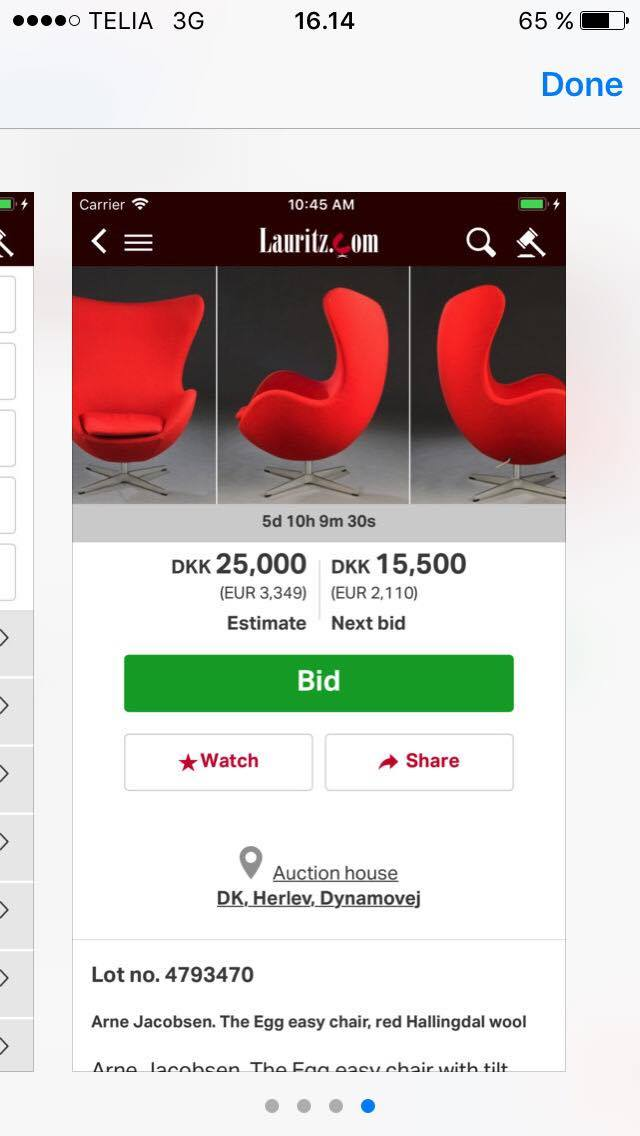
\includegraphics[width=6cm]{Appendix/Lauritzcom.jpg}
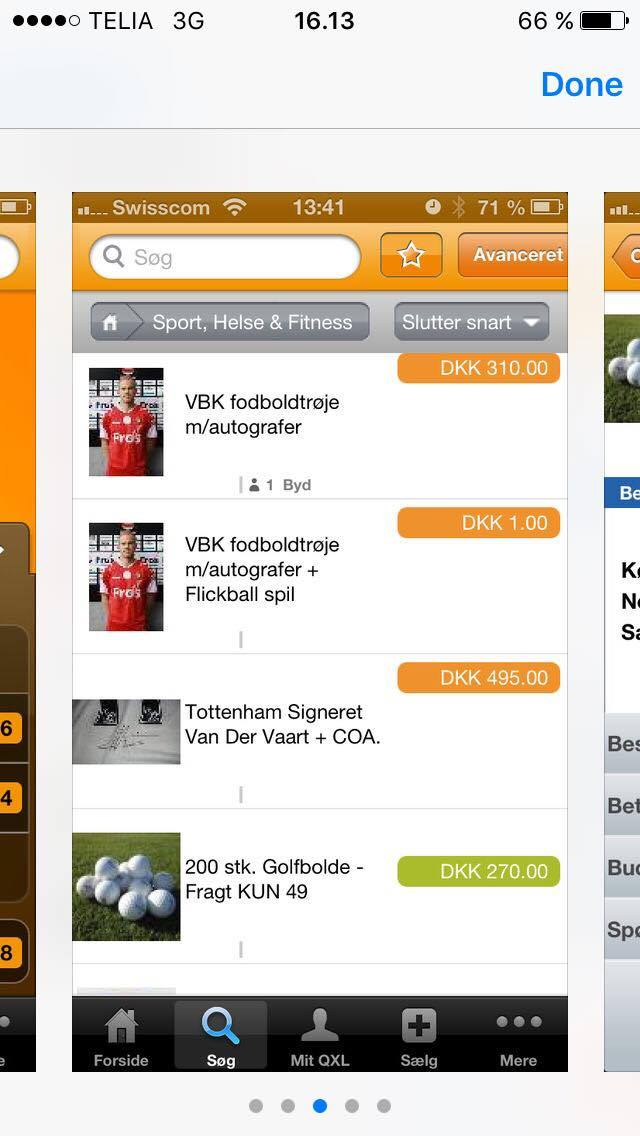
\includegraphics[width=6cm]{Appendix/QXL.jpg}    
\end{center}


\section{Level of market saturation}
Text of Appendix A is Here

\section{Business Models}
\label{Hejsa}
Text of Appendix B is Here

\section{Market Analysis}
Markets demands goes here. 


\end{document}
